\chapter{Categorical Data Representation}
\label{categorical:chapter}

In the previous chapter, we examined the various data models which are widely in use today.
As we saw, there is great variety between the models, and the same thing is true for the query languages designed for their respective models.

In this chapter, we will explore a concrete unified representation~\cite{unified_representation}\cite{one_model} of multi-model data using category theory, a powerful branch of mathematics which studies mathematical structures and relations between them.
We will also discuss the benefits of such a representation, and we will then utilise it to build a universal, multi-model query language.

\section{Benefits of a Unified Representation}

As discussed in~\cref{multimodel}, there already exist two approaches to encompassing multiple data models in a single database system -- polystores~\cite{polystores}\cite{polystores2} and multi-model database systems~\cite{multimodel_dbs}\cite{multimodel_dbs2}.
However, neither approach provides a true, seamless, multi-model experience in terms of data modeling, querying and management, or this experience is only limited to two or three select models~\cite{multimodel_dbs2}.
Naturally, it would be beneficial to be able to work with all popular models in such a unified way.
Ideally, such a unified representation allows us to do the following~\cite{unified_representation}:

\begin{enumerate}
    \item capture all the existing models, preferably in the same and definitely in a standard way; 
    \item query across multiple interconnected models efficiently; 
    \item perform correct and complete evolution management, i.e., propagation of changes; 
    \item enable data migration without complex reorganisations; and 
    \item permit integration of new data models.
\end{enumerate}

Specifically, for the purposes of this thesis, having such a unified representation of multi-model data would form the perfect base for designing a multi-model query language.
This is why we will spend a short while examining the unified representation of multi-model data proposed by Martin Svoboda, Pavel Koupil and Irena Holubov{\'a}~\cite{unified_representation}\cite{one_model}.
To demonstrate the concepts that we will explain in this chapter, we present a sample multi-model scenario in~\cref{fig:datamodel}, with a corresponding Entity Relationship (ER) schema shown in~\cref{fig:erschema}. 

\begin{figure}[ht]
\centering
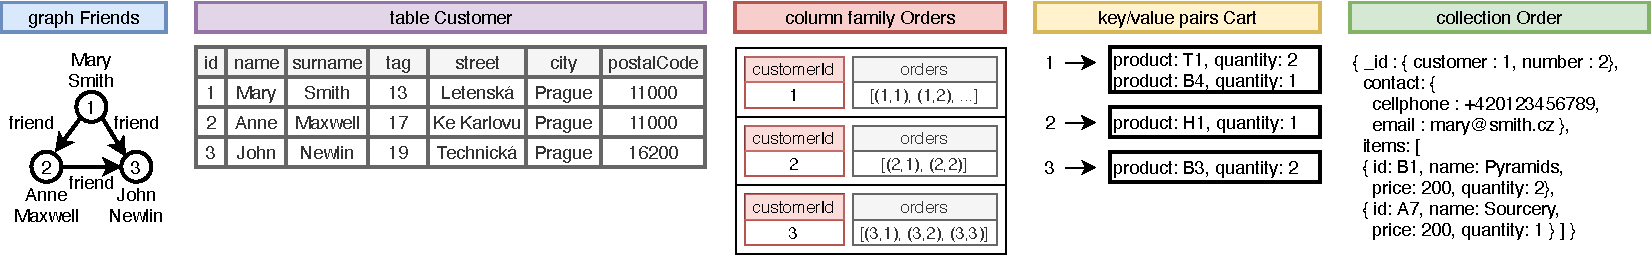
\includegraphics[width=\textwidth]{img/fig_data-models.pdf} 
\caption{A sample multi-model data scenario~\cite{unified_representation}.}
\label{fig:datamodel}
\end{figure}

\section{Basics of Category Theory}

As mentioned earlier, category theory~\cite{category_theory} is a branch of mathematics which
studies mathematical structures and relations between them.
A category $\mathbf{C} = (\mathcal{O}, \mathcal{M}, \circ)$ consists of three entities:

\begin{itemize}
    \item A class $\mathcal{O}$, whose elements are called objects. This class may also alternatively be referred to as $Obj(\mathbf{C})$.
    \item A class $\mathcal{M}$, whose elements are called morphisms, each of which has a target object and a source object. This class may also alternatively be referred to as $Hom(\mathbf{C})$.
    \item A binary operation $\circ$ called the composition over morphisms.
\end{itemize}

A useful visualization form of a category is the form of a \textit{multigraph}, with category objects forming its set of vertices and schema morphisms forming directed edges.

We represent morphisms $f \in \mathcal{M} : A \rightarrow B$, as arrows, with $A, B \in \mathcal{O}$.
We refer to object $A$ as the \textit{domain} of morphism $f$ and to object $B$ as its \textit{codomain}\footnote{The domain and codomain may also be referred to by \textit{dom} and \textit{cod}.}.
Let $f : A \rightarrow B, g : B \rightarrow C \in \mathcal{M}$ be morphisms, then the composite morphism $g \circ f \in \mathcal{M}$ is also part of the set of morphisms in the same category, also called the \textit{transitivity} property.
The morphism composition operation is not only transitive, but it is also \textit{associative}, i.e., $h \circ (g \circ f) = (h \circ g) \circ f$ for any morphisms $f, g, h \in \mathcal{M}$ such that $f : A \rightarrow B, g : B \rightarrow C$, and $h : C \rightarrow D$.
Finally, for every object $A \in \mathcal{O}$, an \textit{identity} morphism $1_A$ must exist, where $f \circ 1_A = f = 1_B \circ f$ for any $f : A \rightarrow B$.
With respect to the composition operation, this identity morphism therefore acts as a unit element.

\begin{figure}[ht]
\centering
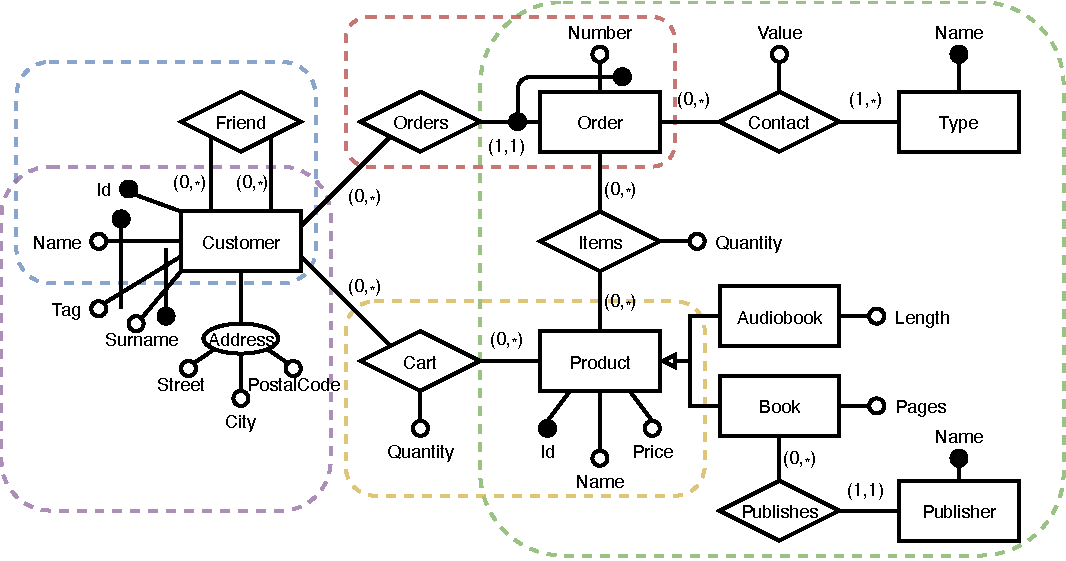
\includegraphics[width=\textwidth]{img/fig_schema-er.pdf} 
\caption{ER schema of the sample multi-model scenario in Figure~\ref{fig:datamodel}~\cite{unified_representation}.}
\label{fig:erschema}
\end{figure}

With these basic concepts from category theory, we can introduce the unified model~\cite{one_model}\cite{unified_representation} which we will be using in the rest of this thesis.
We will introduce three main concepts which together form the basis of this model -- the \textbf{schema category} describing the schema of the data in question, the \textbf{instance category} describing actual data conforming to its corresponding schema category, and the \textbf{mappings} which describe how objects from the schema category are stored in the underlying databases.
Note that the introduction of the following concepts is somewhat informal and does not cover every single aspect of the categorical model, and for this reason we refer the reader to the original sources on the matter~\cite{one_model}\cite{unified_representation} for a more comprehensive definition.

\section{Schema Category}
\label{categorical:section:schema}

We define a \textit{schema category}~\cite{one_model}\cite{unified_representation} as a tuple  $\mathbf{S} := (\mathcal{O}_\mathbf{S}, \mathcal{M}_\mathbf{S}, \circ_\mathbf{S})$, with $\mathcal{O}$ being the set of \textit{schema objects}, $\mathcal{M_\mathbf{S}}$ being the set of schema morphisms, and $\circ$ being the morphism composition operation.
Schema morphisms in $\mathcal{M}_\mathbf{S}$ connect pairs of objects from $\mathcal{O_\mathbf{S}}$.
We distinguish two types of morphisms in $\mathcal{M}_\mathbf{S}$:

\begin{itemize}
    \item \textit{Base} morphisms are morphisms which are explicitly defined; and
    \item \textit{Composite} morphisms which are obtained via the composition of base or composite morphisms via the composition operation $\circ$.
\end{itemize}

We define each schema object $o := (key$, $label$, $superid$, $ids) \in \mathcal{O}_\mathbf{S}$ to be a tuple.
Let $\mathbb{O} \subseteq \mathbb{N}$ be a set of numbers forming the set of object identifiers.
Then $key \in \mathbb{O}$ is an automatically assigned object identifier, unique for each schema object.
We can optionally define names for schema objects using the $label$ property, which is defined as $\bot$ when missing.
Naturally, we also need our schema to contain the model of the data it represents.
For this reason, each object contains a set of attributes $superid \ne \emptyset$, where each attribute corresponds to a morphism signature, introduced in the following paragraph.
The set $superid$ models the data each object is expected to contain.
Finally, the set $ids \ne \emptyset \subseteq \mathcal{P}(superid)$ is a set of identifiers, each being a set of attributes from $superid$.
This allows us to uniquely distinguish individual data instances using their attributes.

\def\myConcat{\!\cdot\!}

Each morphism $m := (signature$, $dom$, $cod$, $min$, $max) \in \mathcal{M}_\mathbf{S}$ is also defined as tuple, regardless of whether the morphism is base or composite.
Firstly, let us define the alphabet $\mathbb{M}$, and the set of possible strings $\mathbb{M}^{*}$ over this alphabet (including $\varepsilon$ which denotes an empty string).
These strings are ordered lists of symbols from $\mathbb{M}$, concatenated using the $\cdot$ operator (for example $1$ for a string containing a single character, $1.2.3$ for a string with three characters, and $\varepsilon$ for an empty string).
For a given morphism $m$, $signature \in \mathbb{M}^{*}$ uniquely identifies this morphism, save for all identity morphisms which share the $\varepsilon$ signature.
If $m$ is a base morphism, its signature will be a single alphabet symbol, i.e. $signature \in \mathbb{M}$.
If $m$ is a composite morphism however, its signature will be a string $signature \in \mathbb{M}^{*} \setminus (\mathbb{M} \cup \{\varepsilon\})$, as this allows us to decompose a composite morphism into its constituent base morphisms according to the $\circ$ operation.
The domain and codomain of $m$ are represented by $dom$ and $cod$ respectively, with both referring to schema objects in $\mathcal{O}$.
In order to model the cardinality of each morphism, we also have the properties $min \in \{\mathtt{0}, \mathtt{1}\}$ and $max \in \{\mathtt{1}, \mathtt{*}\}$, which specify the minimal and maximal number of occurrences of each specific morphism in the instance category respectively.

\begin{figure}[!htb]
\centering
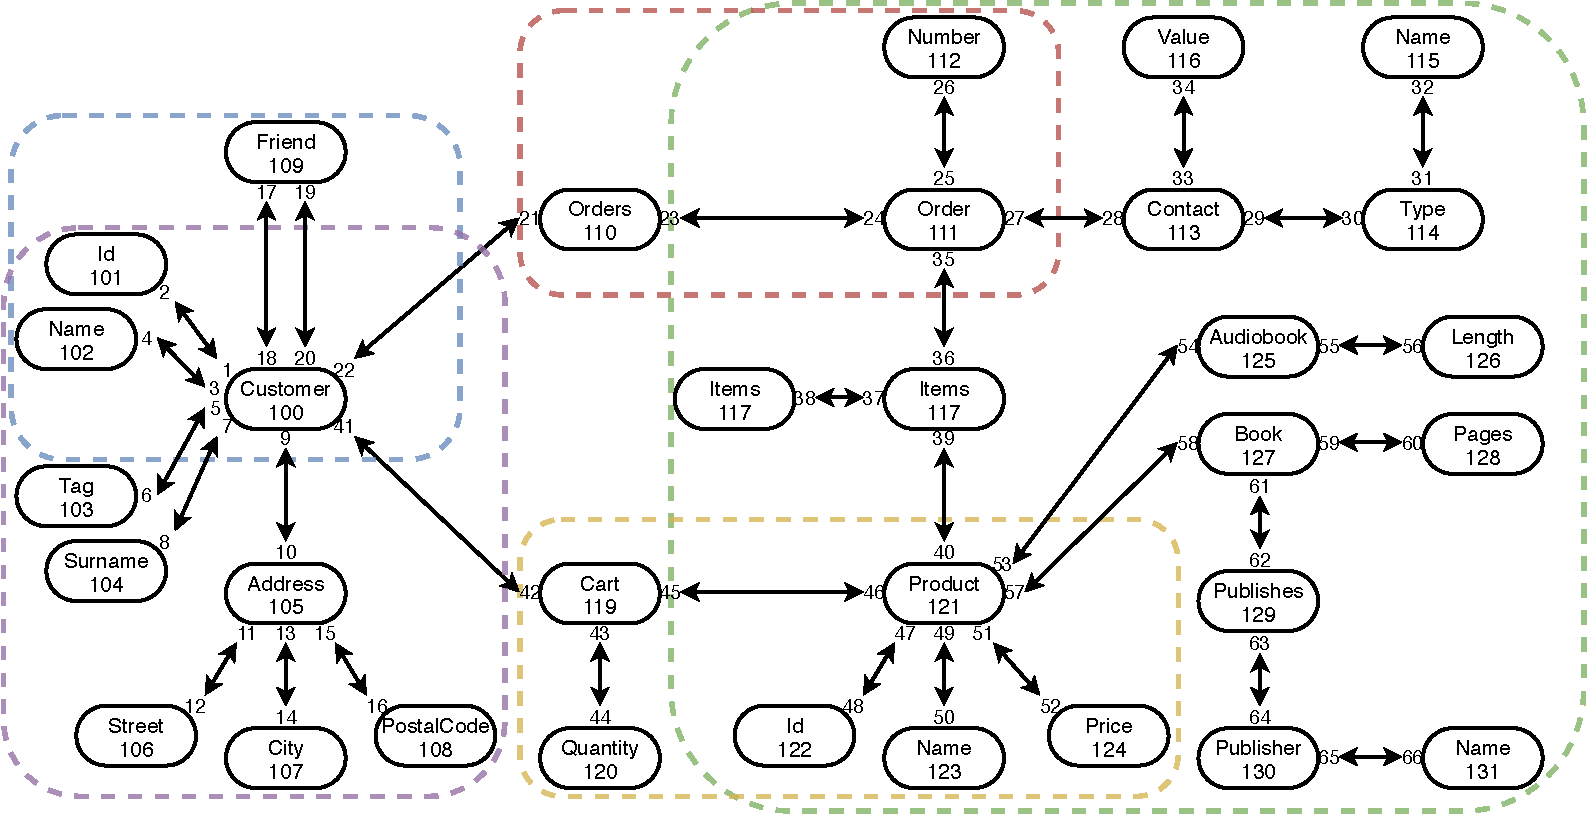
\includegraphics[width=\textwidth]{img/fig_schema-categorical.pdf} 
\caption{Schema category which was extracted from the sample ER schema in \cref{fig:erschema}~\cite{unified_representation}.}
\label{fig:schemacategory}
\end{figure}

When it comes to morphism composition, we define the signature of the composite morphism $m_2 \circ m_1$ to be $signature := signature_2\myConcat signature_1$, unless either morphism is an identity morphism, in which case the resulting signature is the signature of the other morphism.
The domain and codomain are composed naturally, resulting in the composite morphism having the domain of $m_1$ and codomain of $m_2$.
Finally, we define the composite cardinalities to be  $min = \min(min_1, min_2)$ and $max = \max(max_1, max_2)$.
With the necessary definitions out of the way, we present an example of a schema category in \cref{fig:schemacategory}, where we can see the schema category corresponding to the sample multi-model scenario presented earlier in \cref{fig:datamodel}.

\section{Instance Category}
\label{categorical:section:instance}

As we mentioned earlier, the schema category $\mathbf{S}$ only describes the schema of the data, not data instances themselves.
For this, we need to introduce the notion of an \textit{instance category}~\cite{one_model}\cite{unified_representation}.
An instance category $\mathbf{I} = (\mathcal{O}_\mathbf{I}, \mathcal{M}_\mathbf{I},$ $\circ_\mathbf{I})$ has the same structure as the corresponding schema category $\mathbf{S}$, meaning that for each schema object and morphism in $\mathbf{S}$, there exists a corresponding instance object or morphism in $\mathbf{I}$ and vice versa.
A particular instance category $\mathbf{I}$ describes the data stored in a set of databases at a particular point in time, being essentially a snapshot of the entire data set.
Whenever the underlying data changes, this will naturally induce a new instance category, with the relevant changes reflected.

Even though the sets of objects $\mathcal{O}_\mathbf{S}$ and $\mathcal{O}_\mathbf{I}$ have the same structure, just like $\mathcal{M}_\mathbf{S}$ and $\mathcal{M}_\mathbf{I}$, their representation must necessarily differ in order to be able to model the data instance.
Let $\mathbb{V}$ be a set of all possible primitive values within the data instance we are describing.
Then each instance object $o_\mathbf{I} := \{t_1, t_2, \dots, t_n\} \in \mathcal{O}_\mathbf{I}$ is a set of tuples $t_i: superid \rightarrow \mathbb{V}$ for all $i \in \mathbb{N}, 0 < i \leq n$, specifying the concrete values this instance object has in the current data instance.
The specific set of tuples defined for a particular data instance for an instance object $o_\mathbf{I} \in \mathcal{O}_\mathbf{I}$ is called the \textit{active domain} of this instance object, meaning the set of data currently bound to it.

Recall that each schema object also contains a set of identifiers $ids$, each of which uniquely identifies a particular object instance.
In an instance category, this unique identification property must hold for each $id \in ids$ for each $o_\mathbf{I} \in \mathcal{O}_\mathbf{I}$.
This means that if we project the active domain of this object to any particular identifier of this object, the number of unique tuples in the active domain must not change.

Now that we have explained the notion of instance objects when compared to schema objects, let us also introduce \textit{instance morphisms}, which act as binary relations between instance object active domains.
Let us consider an instance morphism $m_\mathbf{I} \in \mathcal{M}_\mathbf{I}$, $m_\mathbf{I} : o_1 \rightarrow o_2$ for some objects $o_1, o_2 \in \mathcal{O}_\mathbf{I}$.
Then $m_\mathbf{I} \subseteq o_1 \times o_2$, meaning that the morphism is a subset of the relation induced by the Cartesian product of $o_1$ and $o_2$ (meaning the product of their active domains).
Note that even though we define morphisms to be directed, we can traverse them in the opposite direction as they are defined as relations, which will be useful to us later.

\section{Mapping Data to the Categorical Representation}
\label{categorical:section:mapping}

In the previous sections, we defined the notion of a schema category representing the data schema, and an instance category representing the entire set of data at a particular point in time.
However, in order to be able to automatically transition between the native data model and the categorical model, we also need to know how they map to each other.
For this reason, we introduce the notion of \textit{mappings}~\cite{unified_representation}, which specify how data for one or more schema objects and morphisms are stored within a particular kind (recall \cref{table:datamodels:terms}) for a particular database.
For example, this could mean describing the structure of rows in a table in the relational model, the structure of documents in a collection in the document model, or the structure of objects and their relationships in the graph model and so on.
As it is likely that the entire schema will not fit within a single kind of a single database, it is expected that there will be multiple mappings for any given schema category, possibly even with some degree of overlap between the mappings if data redundancy is present.
These mappings may be created manually by the user using a tool like MM-evocat~\cite{evocat} which we will be working with later in this thesis, but there are also approaches which attempt to infer the mapping from the databases themselves like MM-infer~\cite{mm_infer}.
Note that sometimes, we may use the terms mapping and kind interchangeably in this thesis (especially during algorithmic descriptions), but in those cases we are always referring to the mapping which maps a given kind to its categorical representation.

% We don't consider root morphisms at all, maybe I should add some explanation for why we don't? Pavel Koupil said it was not necessary IIRC but I don't remember the reasoning.
Each of these mappings consists of a root object, denoting the root of the context of this kind within the schema category, the name of the kind which this mapping corresponds to, the source database of the kind, and finally an \textit{access path}, which describes the internal structure of the kind, and its mapping to the categorical representation.
The access path for any given kind has a tree-like structure rooted in the mapping's root object, and recursively specifies the shape of the kind.
We generally use a JSON-like representation of the access path, as shown in \cref{fig:mappings}.

\begin{figure}[ht]
\centering
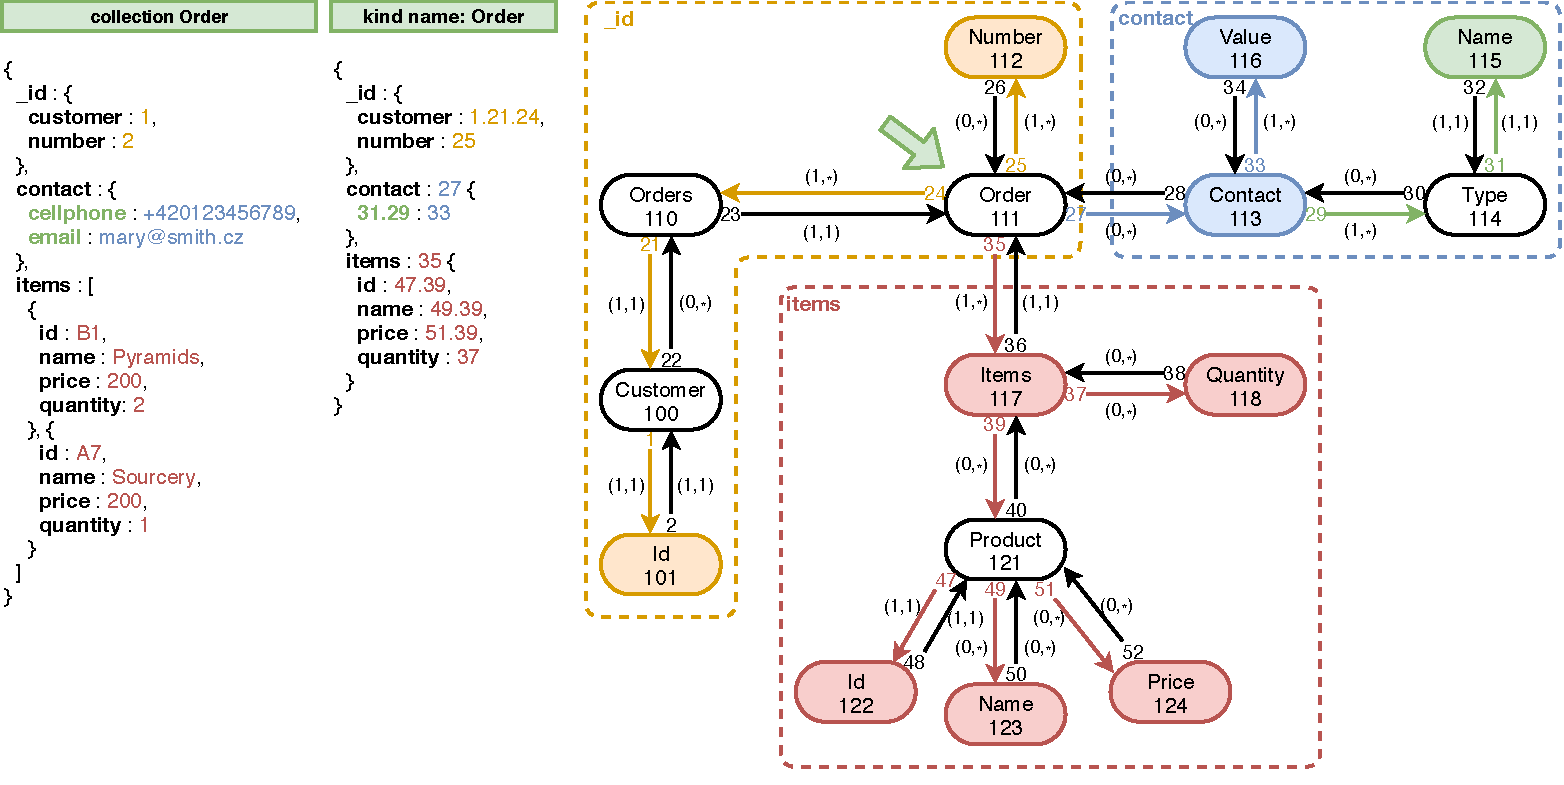
\includegraphics[width=\textwidth]{img/fig_access-path-data.pdf} 
\caption{Collection \textit{Order}, an access path for kind \textit{Order}, and the corresponding part of schema category $\mathbf{S}$~\cite{unified_representation}}
\label{fig:mappings}
\end{figure}

When defining a property within the access path, we always define its name and structure, where the structure is constrained by the particular database model (for instance, mappings for kinds in a purely relational database are always flat with no nested properties, and their property names must be unique).
This structure in the form of an access path must always cover at least one identifier of the root object, as without it, it would not be possible to distinguish different object instances.
We will point out that not every schema object needs to be the root object of a mapping, as mappings generally map the values of many schema objects which are specified within a single mapping (for example the set of customer names, surnames and ids from a single relational table).

We distinguish three possibilities for the kinds of child properties in the access path for a given mapping:

\begin{itemize}
    \item The child property is a direct neighbour of its parent in the schema category, meaning it is accessible via a base morphism.
    \item The child property is \textit{inlined} from a more distant position within the schema category, meaning it is accessible from its parent via a composite morphism. Note that multiple paths can exist in the schema category between any given objects, which is why the exact composition of the composite morphism is important.
    \item The child property is \textit{auxiliary}, meaning no corresponding object exists in the schema category. The purpose of such properties is purely structural.
\end{itemize}

The aforementioned associated morphisms are also called the property \textit{context}, as they determine which schema object each property maps to (if any).
Properties can have other kinds of names than simple static names, specifically we distinguish the following possibilities:

\begin{itemize}
    \item \textit{Static} names are user-defined as required by the structure of the underlying kind;
    \item \textit{Dynamic} names are derived from instances of particular schema objects (for example types of contact like phone or email within a customer contact object); and
    \item \textit{Anonymous} properties which do not have a name, or their naming is not permitted within the given model (for example array elements in JSON).
\end{itemize}

When it comes to the values of properties, we distinguish only two types of values:

\begin{itemize}
    \item \textit{Simple} properties which only contain primitive values; and
    \item \textit{Complex} properties containing a set or list of child properties, like a nested array or nested object in JSON. 
\end{itemize}

Note that the explanation of the concept of mappings was considerably less formal than the ones for schema and instance categories, as the formal definition is more complex in the case of mappings.
For a more formal definition of the concept of a mapping, please refer to the paper by Pavel Koupil and Irena Holubov{\'a}, where an exact definition is given~\cite{unified_representation}. 
While reading the original proposal of these ideas is not strictly necessary for readers of this thesis, it will certainly make the rest of it more digestible, as we will be expecting a certain level of familiarity with these concepts.

\section{The Need for a Categorical Query Language}
\label{category:section:querylanguage}

Now that we have examined the basics of category theory and the unified model we will be considering in the rest of this thesis, let us consider the \textit{why} of building a query language using this unified model.
As discussed earlier, there is no standard truly multi-model query language, which would be able to uniformly encompass all currently popular data models.
The utility of such a query language should be fairly apparent -- one does not need to bother with a different query language for each subset of their data which happens to be stored in a database with a different paradigm.
On the contrary, queries across the entirety of one's data may easily be expressed in the same query language.

Even in the situation where one is not particularly perturbed by the need to know multiple query languages, there are still a few more problems on the horizon.
Namely, there is an issue with queries which cross the boundaries of multiple database systems.
For example, let us consider a scenario where we store a table of user information in PostgreSQL, and we store the order information in a collection in MongoDB.
In such a case, expressing a query which crosses the boundaries of both databases is impossible without sharing the same query language.

As the reader now hopefully shares our enthusiasm for the existence of such a language, we must still formalize the requirements for such a language.
This language should:

\begin{itemize}
    \item be able to encompass the particulars of all popular data models,
    \item be able to express queries crossing model boundaries,
    \item be expressive and readable,
    \item leverage the power of category theory,
    \item be intuitive and familiar to users of existing query languages,
    \item have the capability of being nearly as performant as native queries where possible.
\end{itemize}

Considering we may look at a category as a multigraph, we may not need to create a categorical query language from scratch.
We can attempt to take inspiration in existing graph query languages, which is the focus of the following chapter.
